\documentclass[border=3mm]{standalone} 
\usepackage{tikz}
\usetikzlibrary{calc}
\usepackage{tkz-euclide}

\begin{document}

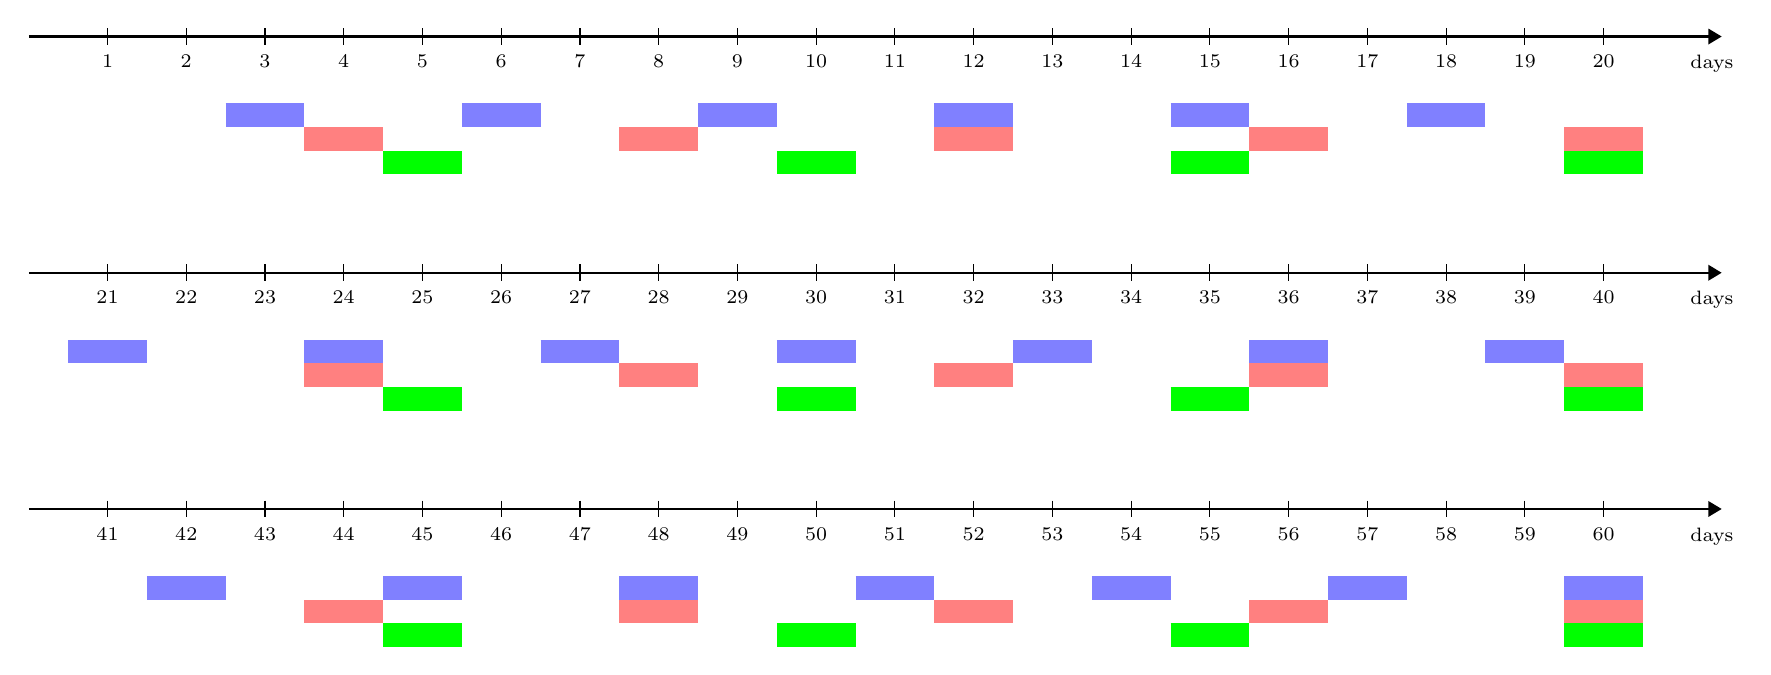
\begin{tikzpicture}

\begin{scope}

% draw horizontal line   
\draw[thick, -Triangle] (0,0) -- (21.5,0) node[font=\scriptsize, below left=3pt and -8pt]{days};

% draw vertical lines
\foreach \x in {1,...,20}
  \draw (\x,3pt) -- (\x,-3pt);

% label vertical lines
\foreach \x in {1,...,20}
  \node[font=\scriptsize, text height=1.75ex, text depth=.5ex]% 
    at (\x,-.3) {$\x$};

% soccer
\foreach \x in {3,6,...,18}
  \draw[blue!50, line width=0.3cm] (\x-0.5,-1.0) -- +(1,0);

% basketball
\foreach \x in {4,8,...,20}
  \draw[red!50, line width=0.3cm] (\x-0.5,-1.3) -- +(1,0);

% volleyball
\foreach \x in {5,10,15,20}
  \draw[green, line width=0.3cm] (\x-0.5,-1.6) -- +(1,0);

\end{scope}


\begin{scope}[yshift=-3cm]

% draw horizontal line
\draw[thick, -Triangle] (0,0) -- (21.5,0) node[font=\scriptsize, below left=3pt and -8pt]{days};

% draw vertical lines
\foreach \x in {21,...,40}
  \draw (\x-20,3pt) -- (\x-20,-3pt);

% label vertical lines
\foreach \x in {21,...,40}
  \node[font=\scriptsize, text height=1.75ex, text depth=.5ex]% 
    at (\x-20,-.3) {$\x$};

% soccer
\foreach \x in {21,24,...,39}
  \draw[blue!50, line width=0.3cm] (\x-20-0.5,-1.0) -- +(1,0);

% basketball
\foreach \x in {24,28,...,40}
  \draw[red!50, line width=0.3cm] (\x-20-0.5,-1.3) -- +(1,0);

% volleyball
\foreach \x in {25,30,35,40}
  \draw[green, line width=0.3cm] (\x-20-0.5,-1.6) -- +(1,0);

\end{scope}


\begin{scope}[yshift=-6cm]

% draw horizontal line
\draw[thick, -Triangle] (0,0) -- (21.5cm,0) node[font=\scriptsize, below left=3pt and -8pt]{days};

% draw vertical lines
\foreach \x in {41,...,60}
  \draw (\x-40,3pt) -- (\x-40,-3pt);

% label vertical lines
\foreach \x in {41,...,60}
  \node[font=\scriptsize, text height=1.75ex, text depth=.5ex]% 
    at (\x-40,-.3) {$\x$};

% soccer
\foreach \x in {42,45,...,60}
  \draw[blue!50, line width=0.3cm] (\x-40-0.5,-1.0) -- +(1,0);

% basketball
\foreach \x in {44,48,...,60}
  \draw[red!50, line width=0.3cm] (\x-40-0.5,-1.3) -- +(1,0);

% volleyball
\foreach \x in {45,50,55,60}
  \draw[green, line width=0.3cm] (\x-40-0.5,-1.6) -- +(1,0);

\end{scope}

\end{tikzpicture}

\end{document}
